\documentclass[letterpaper]{article}

../../../../tex/scufftex.tex

\graphicspath{{figures/}}

%------------------------------------------------------------
%------------------------------------------------------------
%- Special commands for this document -----------------------
%------------------------------------------------------------
%------------------------------------------------------------

%------------------------------------------------------------
%------------------------------------------------------------
%- Document header  -----------------------------------------
%------------------------------------------------------------
%------------------------------------------------------------
\title {Fresnel Scattering with {\sc scuff-scatter-periodic}}
\author {Homer Reid}
\date {July 24, 2012}

%------------------------------------------------------------
%------------------------------------------------------------
%- Start of actual document
%------------------------------------------------------------
%------------------------------------------------------------

\begin{document}
\pagestyle{myheadings}
\markright{Homer Reid: Fresnel Scattering with {\sc scuff-scatter-periodic}}
\maketitle

\tableofcontents

%%%%%%%%%%%%%%%%%%%%%%%%%%%%%%%%%%%%%%%%%%%%%%%%%%%%%%%%%%%%%%%%%%%%%%
%%%%%%%%%%%%%%%%%%%%%%%%%%%%%%%%%%%%%%%%%%%%%%%%%%%%%%%%%%%%%%%%%%%%%%
%%%%%%%%%%%%%%%%%%%%%%%%%%%%%%%%%%%%%%%%%%%%%%%%%%%%%%%%%%%%%%%%%%%%%%
\newpage
\section{Exact Solution}
%####################################################################%
%####################################################################%
%####################################################################%
\begin{figure}
\begin{center}
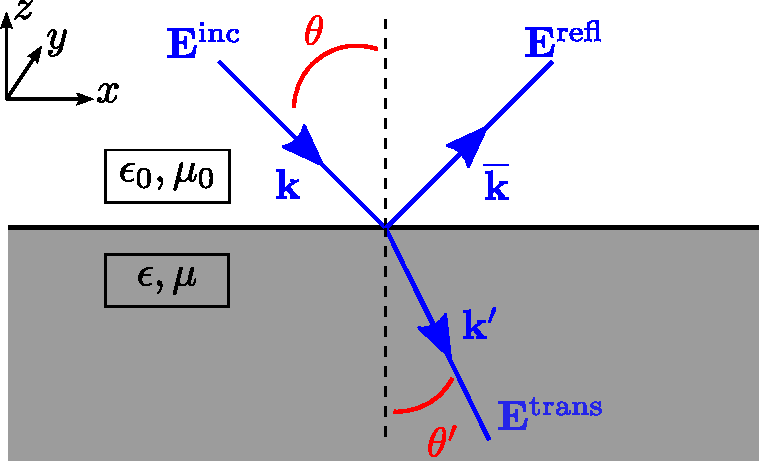
\includegraphics{FresnelCartoon.pdf}
\label{FresnelCartoonFigure}
\caption{Fresnel scattering.}
\end{center}
\end{figure}
%####################################################################%
%####################################################################%
%####################################################################%

Consider a plane wave at frequency $\omega$ impinging on an infinite
planar material surface at incident angle $\theta$ 
(Figure \ref{FresnelCartoonFigure}).

\subsection*{Incident field}

In what follows, the superscripts ``perp'' and ``par'' describe the 
two possible polarizations: $\vb E-$field perpendicular or parallel to 
the plane of incidence.
\begin{align*}
 \vb E\sups{inc,perp}(\vb x) 
  &= E_0 e^{i\vb k \cdot \vb x}\, \vbhat{y} 
\\
 \vb E\sups{inc,par}(\vb x) 
  &= E_0 e^{i\vb k \cdot \vb x} 
     \Big(\cos\theta\,\vbhat{x} + \sin\theta\,\vbhat{z}\Big)
\end{align*}
where 
$$ \vb k=k\Big(\sin\theta\,\vbhat{x} - \cos\theta\,\vbhat{z}\Big), 
   \qquad 
   k=\frac{\omega}{c}.
$$

\subsection*{Bloch wavevector}

The Bloch wavevector $\vb p$ that we will specify to 
{\sc scuff-scatter-periodic} depends on the incident 
angle. To identify this dependence, we note that the
phase factor in the expression for the incident field 
is 
$$ e^{i\vb k \cdot \vb x} = e^{ik (x\sin\theta - z\cos\theta)}$$
Hence, for an arbitrary in-plane (two-dimensional) lattice 
vector $\vb L=L_x\vbhat{x}+L_y\vbhat{y}$, both 
$\vb E\sups{inc,perp}$ and $\vb E\sups{inc,par}$ satisfy the condition
$$ 
 \vb E(\vb x+\vb L) = e^{ik\sin\theta L_x} \vb E(\vb x)
$$ 
whereupon we identify the Bloch wavevector as 
$$ \vb p = (p_x, p_y) = (k\sin\theta, 0).$$

%%%%%%%%%%%%%%%%%%%%%%%%%%%%%%%%%%%%%%%%%%%%%%%%%%%%%%%%%%%%%%%%%%%%%%
%%%%%%%%%%%%%%%%%%%%%%%%%%%%%%%%%%%%%%%%%%%%%%%%%%%%%%%%%%%%%%%%%%%%%%
%%%%%%%%%%%%%%%%%%%%%%%%%%%%%%%%%%%%%%%%%%%%%%%%%%%%%%%%%%%%%%%%%%%%%%
\subsection*{Scattered fields}

\subsubsection*{Reflected fields}

We refer to the scattered fields in the region $z>0$ 
as the ``reflected`` fields:
\begin{subequations}
\begin{align}
 \vb E\sups{perp,refl}(\vb x)
  &= -r\sups{perp} E_0 \, e^{i\overline{\vb k}\cdot \vb x} \, \vbhat{y} 
\\
 \vb E\sups{par,refl}(\vb x) 
  &= -r\sups{par} E_0 e^{i\overline{\vb k}\cdot \vb x} 
     \left(\cos\theta\,\vbhat{x} - \sin\theta\,\vbhat{z}\right)
\end{align}
\label{Erefl}
\end{subequations}
where $\overline{\vb k}$ is the incident wavevector with its
$z$ component flipped:
$$ \overline{\vb k}= k\Big(\sin\theta\,\vbhat{x} + \cos\theta\,\vbhat{z}\Big).$$

\subsubsection*{Transmitted fields}

The fields in the region $z<0$ are the ``transmitted`` fields:
\begin{subequations}
\begin{align}
 \vb E\sups{perp,trans}(\vb x)
  &= t\sups{perp}E_0\vbhat{y} e^{i\vb k^\prime\cdot \vb x}
\\
 \vb E\sups{par,trans}(\vb x) 
  &= t\sups{par} E_0\left(\cos\theta^\prime\vbhat{x} + \sin\theta^\prime\vbhat{z}\right)
  e^{i\vb k^\prime \cdot \vb x} 
\end{align}
\label{Etrans}
\end{subequations}

The transmitted wavevector is 
$$ \vb k^\prime= \sqrt{\epsilon \mu} \cdot k 
   \Big(\sin\theta^\prime\vbhat{x} - \cos\theta^\prime\vbhat{z}\Big)
$$
with the refraction angle defined by 
$$ \sin \theta^\prime = \frac{\sin\theta}{\sqrt{\epsilon\mu}}.$$

%%%%%%%%%%%%%%%%%%%%%%%%%%%%%%%%%%%%%%%%%%%%%%%%%%%%%%%%%%%%%%%%%%%%%%
%%%%%%%%%%%%%%%%%%%%%%%%%%%%%%%%%%%%%%%%%%%%%%%%%%%%%%%%%%%%%%%%%%%%%%
%%%%%%%%%%%%%%%%%%%%%%%%%%%%%%%%%%%%%%%%%%%%%%%%%%%%%%%%%%%%%%%%%%%%%%
\subsubsection*{Reflection and transmission coefficients}

$$\begin{array}{lclclcl}
  t\sups{perp} 
  &=& 
  \displaystyle{\frac{2Z\cos\theta}{Z\cos\theta + \cos\theta^\prime}}
  &\qquad&
  r\sups{perp} 
  &=& 
  \displaystyle{\frac{Z\cos\theta - \cos\theta^\prime}{Z\cos\theta + \cos\theta^\prime}}
\\[15pt]
  t\sups{par} &=& 
  \displaystyle{\frac{2Z\cos\theta}{\cos\theta + Z\cos\theta^\prime}}
  &\qquad&
  r\sups{perp} &=& 
  \displaystyle{\frac{\cos\theta - Z\cos\theta^\prime}{\cos\theta + Z\cos\theta^\prime}}
\end{array}
$$
with
$$ Z=\sqrt\frac{\mu}{\epsilon}.$$

%%%%%%%%%%%%%%%%%%%%%%%%%%%%%%%%%%%%%%%%%%%%%%%%%%%%%%%%%%%%%%%%%%%%%%
%%%%%%%%%%%%%%%%%%%%%%%%%%%%%%%%%%%%%%%%%%%%%%%%%%%%%%%%%%%%%%%%%%%%%%
%%%%%%%%%%%%%%%%%%%%%%%%%%%%%%%%%%%%%%%%%%%%%%%%%%%%%%%%%%%%%%%%%%%%%%
\newpage
\section{Solution using {\sc scuff-scatter-periodic}}

\subsection{Creating the surface mesh}

\subsection{Specifying field evaluation points}

We will extract the reflection and transmission coefficients 
by evaluating the scattered fields above and below the 
plane and comparing against the expected expressions
(\ref{Erefl}) and (\ref{Etrans}).

More specifically, if $\vb x$ is an 
evaluation point \textit{above} the plane, then we can extract the
reflection coefficients from the scattered $\vb E$-field at $\vb x$
according to 
\begin{align*}
 r\sups{perp} 
 &= -\frac{\vbhat{y} \cdot \vb E\sups{scat,perp}(\vb x)}
          {E_0 e^{i\overline{\vb k}\cdot \vb x}}
\\[5pt]
 r\sups{par} 
 &= -\frac{ (\cos\theta\,\vbhat{x} - \sin\theta\,\vbhat{z})
            \cdot \vb E\sups{scat,par}(\vb x)}
          {E_0 e^{i\overline{\vb k}\cdot \vb x}},
\end{align*}
while if $\vb x$ is an evaluation point \textit{below} the 
plane then we can extract the transmission coefficients from the 
scattered $\vb E$-field at $\vb x$ according to 
\begin{align*}
 t\sups{perp} 
 &= \frac{\vbhat{y} \cdot \vb E\sups{scat,perp}(\vb x)}
         {E_0 e^{i\vb k^\prime \cdot \vb x}}
\\[5pt]
 t\sups{par} 
 &= \frac{ (\cos\theta^\prime\,\vbhat{x} + \sin\theta^\prime\,\vbhat{z})
            \cdot \vb E\sups{scat,par}(\vb x)}
         {E_0 e^{i\vb k^\prime\cdot \vb x}}.
\end{align*}

Here $\vb E\sups{scat,perp}$ and $\vb E\sups{scat,par}$ are the 
scattered fields that result from solving the scattering problem
with incident fields respectively perpendicular and parallel to 
the plane of scattering.

\end{document}
